\documentclass[10pt,UTF8]{ctexart}


\usepackage[margin=2cm,a4paper]{geometry}
%\usepackage[left=0.75in,top=0.6in,right=0.75in,bottom=1.0in,a4paper]{geometry}

\setmainfont{Caladea}
%% 也可以選用其它字庫:
% \setCJKmainfont[%
%   ItalicFont=AR PL KaitiM GB,
%   BoldFont=Noto Sans CJK SC,
% ]{Noto Serif CJK SC}
% setCJKsansfont{Noto Sans CJK SC}
% \renewcommand{\kaishu}{\CJKfontspec{AR PL KaitiM GB}}

% 繁體中文
\setCJKmainfont[Path=fonts/ ]{NotoSansTC-Medium.otf}

\usepackage{minted}
\usepackage[breaklinks]{hyperref}

% Picture
% 導言區的此三行無變化
\usepackage{graphicx}
\usepackage{float} 
\usepackage{subfigure}
% 以下是新增的自定義格式更改
\usepackage[]{caption2} %新增調用的宏包
\renewcommand{\figurename}{Fig.} %重定義編號前綴詞
\renewcommand{\captionlabeldelim}{.~} %重定義分隔符
 %\roman 是羅馬數字編號,\alph是默認的字母編號,\arabic是阿拉伯數字編號,可按需替換下一行的相應位置
\renewcommand{\thesubfigure}{(\roman{subfigure})}%此外,還可設置圖編號顯示格式,加括號或者不加括號
\makeatletter \renewcommand{\@thesubfigure}{\thesubfigure \space}%子圖編號與名稱的間隔設置
\renewcommand{\p@subfigure}{} \makeatother

% Math
\usepackage {mathtools}
\usepackage{amssymb}

% Code
\usepackage{listings}
\usepackage{xcolor}
\lstset{
    % backgroundcolor=\color{red!50!green!50!blue!50},
    % 程式碼塊背景色為淺灰色
    rulesepcolor= \color{gray}, % 程式碼塊邊框顏色
    breaklines=true,  % 程式碼過長則換行
    numbers=left, % 行號在左側顯示
    numberstyle= \small,% 行號字型
    % eywordstyle= \color{red,% 關鍵字顏色
    commentstyle=\color{gray}, % 註釋顏色
    frame=shadowbox % 用方框框住程式碼塊
    }

\usepackage{hyperref}

\title{算法分析和複雜性理論}
\author{干皓丞,2101212850, 信息工程學院}

\begin{document}
\maketitle


\section{作業目標與章節摘要}

1. 背包問題 (Knapsack Problem)

一個旅行者隨身攜帶一個背包,可以放入背包的物品有 n 種,每種物品的重量和價值分別是 $w_{i}$ , $v_j$, $i = 1$, ... , n 。

如果背包的最大容量限制是 b,怎樣選擇放入背包的物品以使得背包的價值最大 ?

2. 投資問題

設有 m 元錢, n 項投資, 函數 $f_{i}(x)$ 表示將 x 元錢投入到第 i 項項目所產生的效益, i=1 ,... , n。

問:如何分配這 m 元錢,使得投資的總效益最高?



\section{作業內容概述}

作業可以從 GitHub 下的 kancheng/kan-cs-report-in-2022 專案找到,作業程式碼與文件目錄為 kan-cs-report-in-2022/AATCC/lab-report/。實際執行的環境與實驗設備為 Google 的 Colab 、MacBook Pro (Retina, 15-inch, Mid 2014) 、 Acer Aspire R7 與 HP Victus (Nvidia GeForce RTX 3060)。本作業 GitHub 專案為 kancheng/kan-cs-report-in-2022 下的 AATCC` 的目錄。程式碼可以從 code 目錄下可以找到 *.pynb,內容包含上次課堂練習、LeetCode 範例思路整理與作業。

https://github.com/kancheng/kan-cs-report-in-2022/tree/main/AATCC

\begin{figure}[H]
\centering 

\includegraphics[width=0.30\textwidth]{aatccqr.png} 
\caption{作業專案位置}
\label{Test}
\end{figure}

\subsection{Demo 方案}

1. OnlineGDB : https://www.onlinegdb.com/ 

%\newpage

\section{背包問題 (Knapsack Problem)}

\subsection{題目}

一個旅行者隨身攜帶一個背包,可以放入背包的物品有 n 種,每種物品的重量和價值分別是 $w_{i}$ , $v_j$, $i = 1$, ... , n 。
如果背包的最大容量限制是 b,怎樣選擇放入背包的物品以使得背包的價值最大 ?


0/1 背包是動態規劃研究的重要問題,因為它提供了許多有用的見解。
給定一組從 1 到 n 編號的 n 個物品,每個物品都有一個重量 wi 和一個值 vi,以及最大重量容量 W,最大化背包中物品的值的總和,使得重量小於或等於背包的容量。

\subsection{天真的解決方案}


讓我們看看天真的解決方案 - 每個項目只有 2 個選擇,要么包含在背包中,要么忽略該項目。
如果包含項目,則通過減少容量 W - vi 並累積項目值來檢查剩餘項目 (N - 1)。否則,在容量和價值不變的情況下檢查剩餘項目 (N - 1)。同樣,下一個項目將有兩個選擇。如果您將其可視化為樹,它將類似於下面的決策樹:

\begin{figure}[H]
\centering 
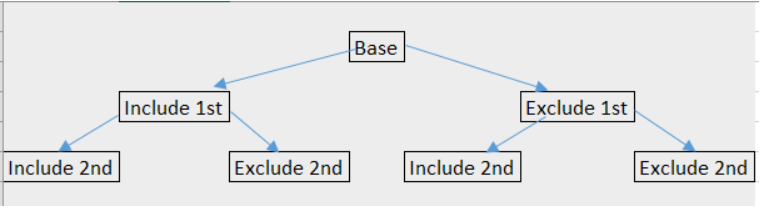
\includegraphics[width=0.90\textwidth]{w6-kp-1.png} 
\caption{圖說明}
\label{Test}
\end{figure}

每個級別 d 有 $2^d$ 個選項,有 N 個項目,因此復雜度為 $2^N$。

另一種將每個項目視為位的方法,然後我們檢查設置和取消設置的所有可能組合,並找到在滿足權重約束時獲得的最大值。很明顯,我們需要檢查 (1 << n) 或 $2^N$ 次迭代。所以,天真的解決方案是 $2^N$。

\subsection{表格法}


考慮一個非常簡單的例子 - 權重 = {1, 2, 3} 和值 ={6, 10, 12},我們有容量為 5 的背包。

現在,讓我們使用表格方法實現相同的功能

\begin{figure}[H]
\centering 
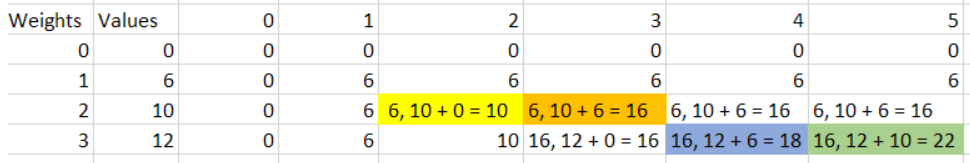
\includegraphics[width=0.90\textwidth]{w6-kp-2.png} 
\caption{表說明}
\label{Test}
\end{figure}

在列上,我們將容量從 0 增加到 W,即最大容量從 0 增加到 5。在每一行上,我們考慮項目,我們注意到它的權重和值。對於每一行,我們只考慮前幾行中考慮的項目,對於每一列,我們考慮那麼多容量。基本情況是重量為 0(無物品),無論容量如何,值都是 0,同樣,如果容量為 0,那麼我們不能放置任何物品,因此值將為 0。

第一行(權重為 1 的行)很簡單,我們的權重為 1,因此我們可以從容量 1 填充它的值。因為只有整行才會有值 6

對於第二行,現在權重為 2,我們可以將與其上方行相同的值填充到容量 2。對於容量 2,它將是 2 選擇 - 包括或排除當前項目。如果我們排除當前項目,則值將與最上面的第 6 行相同。如果我們包括,則值將是 = 當前值 (10) + d(1,當前容量 (2) - 重量(2)) = 10 + d( 1, 2- 2) = 10 + 0 = 10。最大值為 10,因此結果為 10。現在,d 函數是前一項 (1),零權重 = 0。
這就是我們得到公式的方式:


\begin{lstlisting}[language={python}]
d(i, w) = Math.Max( d(i - 1, w), d(i - 1, w - weight[i]) + value[i])
\end{lstlisting}

考慮第 3 行和容量 4,不包括第 3 項,我們從上面的行得到 16 個值,包括它我們發現值 = 12 + d(2, 1) = 12 + 6 = 18。

很明顯,我們對每個容量 0 到 W 和每個項目 0 到 N 只計算一次,所以復雜度是 O(NW)。

參考代碼:

\begin{lstlisting}[language={python}]
// given N, maxWeight, weights and values
long[,] d = new long[N + 1, maxWeight + 1];

for (long i = 0; i < N; i++)
{
	for (long w = 0; w <= maxWeight; w++)
	{                    
		if (weights[i] <= w)
		{
			// Exclude or include
			d[i + 1, w] = Math.Max(d[i, w], d[i, w - weights[i]] + values[i]);
		}

		else
		{
			// Exclude
			d[i + 1, w] = d[i, w];
		}                    
	}
}
\end{lstlisting}

等等,我們如何將時間複雜度從 O(2 \^ N) 提高到 O(N * W)?

這是因為我們重用了已經計算好的解決方案。例如,如果容量 = 7,而不是嘗試不同的項目組合,如 4 + 3、2 + 5、1 + 6、2 + 4 等。我們只做一個計算來排除或包含當前項目。當我們包含當前項目時,我們正在重用已發現容量減少和項目更少的解決方案。

許多動態規劃問題遵循類似的模式,例如

1. 我們有優化功能 - 最大化價值,最小化距離等

2. 最優子結構 - 遞歸地找到子問題的最優解

3. 重疊子問題 - 相同的子問題一次又一次地解決。

動態編程解決每個子問題一次並重用結果。有兩種方法:

1. 自上而下:在子問題的遞歸計算過程中,我們存儲結果,所以當我們再次嘗試子問題時,我們直接使用存儲的結果而不是重新計算。因此,結果應該以可以在 O(1) 時間內檢索到的方式存儲 - 就像使用數組/字典一樣。

2. 自下而上:這裡我們嘗試解決較小的子問題,例如上面的項目和容量,然後到達更大的問題。更大的子問題的解決方案是通過使用已經計算的子問題的解決方案來生成的。

無論哪種情況,我們都需要找出子問題建立的狀態。例如,考慮的項目和剩餘容量是我們的狀態,無論剩餘的項目數量和相同 i 和 w 的總容量如何,我們都具有相同的值。識別狀態對於動態規劃至關重要。


\begin{lstlisting}[language={python}]
from typing import List

def wordBreak(self, s: str, wordDict: List[str]) -> bool:
        bagSize = len(s)+1
        itemSize = len(wordDict)
        dp = [False] * bagSize
        dp[0] = True
        # 排列而不是組合。外遍歷中的背包。
        # 允許重疊物品,背包溯源應從小值開始。
        # 當我們同時遇到一個 True 時中斷
        # Permutation instead of combination. knapsack in outer traversal。
        # Allowed overlapping items,tracersal of knapsack should start with small value。
        # break when we meet a True at once
        for j in range(1, bagSize):
            for i in range(itemSize):
                if j-len(wordDict[i])>=0 and dp[j-len(wordDict[i])] and wordDict[i]==s[j-len(wordDict[i]):j]:                    
                    dp[j] = True
                    break
        return dp[-1]
\end{lstlisting}


\newpage

\section{投資問題}

\subsection{題目}

設有 m 元錢, n 項投資, 函數 $f_{i}(x)$ 表示將 x 元錢投入到第 i 項項目所產生的效益, i=1 ,... , n。

問:如何分配這 m 元錢,使得投資的總效益最高?

\begin{figure}[H]
\centering 
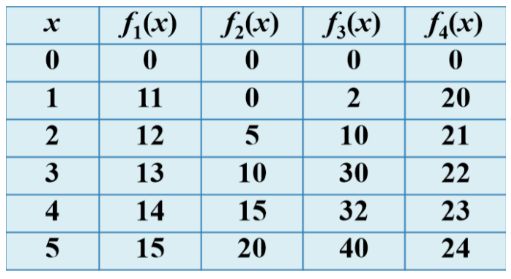
\includegraphics[width=0.90\textwidth]{w6-kp-3.png} 
\caption{事例}
\label{Test}
\end{figure}

\subsection{暴力求解}

算法思想為對所有項目進行循環,通過限定條件:總投資金額 = y,得到所有符合的答案,從中選取最大值,即為所求。

\subsubsection{暴力求解 C++}

\begin{lstlisting}[language={python}]
#include<iostream>
using namespace std;
    //投資問題的暴力解法
int main(){
    int profitMatrix[4][6]={0,11,12,13,14,15,   //收益矩陣
                            0,0,5,10,15,20,
                            0,2,10,30,32,40,
                            0,20,21,22,23,24
    };
    int x1,x2,x3,x4,x;
    int sum=0,maxProfit=0;
    int a[4]={0}; //輸出最優向量
    for(x1=0;x1<6;x1++){
        for(x2=0;x2<6;x2++){
            for(x3=0;x3<6;x3++){
                for(x4=0;x4<6;x4++){
                   x=x1+x2+x3+x4;
                   if(x==5){ //限定條件,投資5萬元
                        sum=profitMatrix[0][x1]+profitMatrix[1][x2]+
                            profitMatrix[2][x3]+profitMatrix[3][x4];
                        if(sum>maxProfit){
                            maxProfit=sum;
                            a[0]=x1;
                            a[1]=x2;
                            a[2]=x3;
                            a[3]=x4;
                        }
                   }
                }
            }
        }
    }
    cout<<"最大利潤為:"<<maxProfit<<endl;
    cout<<"最優投資方案為:( ";
    for(int i=0;i<4;i++){
        cout<<a[i]<<" ";
    }
    cout<<")";
}
\end{lstlisting}

\subsubsection{暴力求解 Python}

\begin{lstlisting}[language={python}]
if __name__ == '__main__':
    profitMatrix=[[0,11,12,13,14,15],
                  [0,0,5,10,15,20],
                  [0,2,10,30,32,40],
                  [0,20,21,22,23,24]]
    a=[0,0,0,0] #存放最優投資方案
    maxProfit=0
    sumMoney=0
    for x1 in range(6):
        for x2 in range(6):
            for x3 in range(6):
                for x4 in range(6):
                    x=x1+x2+x3+x4
                    if x==5:
                        sumMoney=profitMatrix[0][x1]+profitMatrix[1][x2]+profitMatrix[2][x3]+profitMatrix[3][x4]
                    if sumMoney>maxProfit:
                        maxProfit=sumMoney
                        a[0]=x1
                        a[1]=x2
                        a[2]=x3
                        a[3]=x4
    print("最大利潤為:"+str(maxProfit))
    print("最優投資方案為:"+str(a))
\end{lstlisting}

\subsection{動態規劃}

算法思想為假設第 x 個項目投資 m 萬元,則將 x 個項目的 y 萬元投資問題分解為前 x-1 個項目投資 y-m 萬元和第 x 個項目投資 m 萬元。這樣就可以將問題規模減小,直至僅有一個項目,此時的最佳投資方案就是其本身。

令 outspace[x][y] 表示前 x 個項目投資 y 萬元得到的最大利潤,令

profitMatrix[i][m]=fi(m),則動態方程為:

outspace[x][y]=profitMatrix[x][m]+outspace[x-1][y-m]

限定邊界為 outspace[0][k]=profitMatrix[0][k]

\subsubsection{動態規劃 C++}

\begin{lstlisting}[language={python}]
#include<iostream>
using namespace std;

int getProfit(int outspace[4][6],int profitMatrix[4][6],int maxProfit){
    for(int i=0;i<=5;i++){
    //當僅有一個項目時,此項目的收益即為最優,分開賦值是為了避免下面出現 -1 行
        outspace[0][i]=profitMatrix[0][i];
    }
    for(int i=1;i<4;i++){ //逐次加入第2,3,4個項目
        for(int j=0;j<=5;j++){//投資金額
                for(int m=0;m<=j;m++){//m代表最後一個項目投資金額
                    if(outspace[i][j]<profitMatrix[i][m]+outspace[i-1][j-m]){
                        outspace[i][j]=profitMatrix[i][m]+outspace[i-1][j-m];
                        if(outspace[i][j]>maxProfit)
                            maxProfit=outspace[i][j];

                    }
                }
        }
    }
    return maxProfit;
}
int main()
{
    int maxProfit = 0;
    int outspace[4][6]={0};//初始化最大利潤矩陣
    int profitMatrix[4][6]={0,11,12,13,14,15,   //收益矩陣
                            0,0,5,10,15,20,
                            0,2,10,30,32,40,
                            0,20,21,22,23,24
    };
    int a=getProfit(outspace,profitMatrix,maxProfit);
    cout<<"最大收益為:"<<a<<endl;
    return 0;
}
\end{lstlisting}

\subsubsection{動態規劃 Python}

\begin{lstlisting}[language={python}]
def getProfit(profitMatrix,outspace,maxProfit):
    for i in range(6):
        outspace[0][i]=profitMatrix[0][i]
    for i in range(1,4):
        for j in range(6):
            for m in range(j+1):
                if outspace[i][j]<profitMatrix[i][m]+outspace[i-1][j-m]:
                    outspace[i][j]=profitMatrix[i][m]+outspace[i-1][j-m]
                if maxProfit<outspace[i][j]:
                    maxProfit=outspace[i][j]
    return maxProfit
                
if __name__ =='__main__':
    profitMatrix=[[0,11,12,13,14,15],
                  [0,0,5,10,15,20],
                  [0,2,10,30,32,40],
                  [0,20,21,22,23,24]]
    outspace=[]
    for i in range(4):
        outspace.append([])
        for j in range(6):
            outspace[i].append(0)
    maxProfit=0
    a=getProfit(profitMatrix,outspace,maxProfit)
    print("最大利潤為:"+str(a))
\end{lstlisting}

%\newpage

\section{Reference}

1. https://blog.csdn.net/qq\_41580347/article/details/111016310

2. https://www.cxymm.net/article/qq\_41580347/111016310

3. https://web.ntnu.edu.tw/~algo/KnapsackProblem.html

4. https://www.coursera.org/lecture/algorithms/040tou-zi-wen-ti-MbJJj

5. https://leetcode.com/discuss/study-guide/1152328/01-Knapsack-Problem-and-Dynamic-Programming

6. https://leetcode.com/problems/word-break/discuss/1702338/dynamic-programming-knapsack-problem-python-3

7. https://blog.csdn.net/littleshi00/article/details/105397192

8. https://icode.best/i/18557543908876





%\section{附錄}

% 數學意義說明

% $$\min \limits_{G}\max \limits_{D}{V_I(D,\ G)=V(D,G)-\lambda L_I(G,Q)}$$

%	\begin{lstlisting}[language={python}]

%	\end{lstlisting}

%\begin{enumerate}
%\item Y
%\item A
%\end{enumerate}

% \newpage

\clearpage

\end{document}